%%%%%% General %%%%%%%%%%%%%%%%%%%%%%%%%%%%%%%%%%%%%%%%%%%%%%%%%%%%%%%%%%%%%%{{{
\chapter{General}\label{sec:general}

This chapter describes terms, techniques, tools and programs used during the
work for this thesis. It provides a general overview to make it easier to
understand the details of the work in the following chapters.

\section{ELF - Executable and Linkable Format}

The ELF format is an object file format. It is used to describe a program in a
way to execute it on a processor without applying changes to the binary itself.
The assembler and linker create the ELF files. The ELF
specification~\cite{elfspec} is followed by most modern Unix like operating
systems, therefore we need to understand the layout of the executable files
before introducing bitflips to it.

\subsection{Structure of an ELF file}

There are two views of an ELF binary, the so called linking view and the the 
execution view. Those views are also called section and segment view. They 
share the same ELF header but serve different purposes for the operating system.

\subsubsection{Sections}

Sections describe the binary for the linking view, it contains instructions,
data, symbol table and relocation information. Sections reserved for the system
start with a dot, there might be additional sections defined by the user.
Sections that are directly loaded into the program's memory image are
initialized data (\texttt{.data, .data1}), read-only data (\texttt{.rodata,
.rodata1}) and executable instructions (\texttt{.text}).

\subsubsection{Segments}

Segments describe the virtual memory layout of a loaded binary. The so called 
process image contains segments with \texttt{text}, \texttt{data}, 
\texttt{stack} and others. When loading the image into memory references inside 
the ELF file need to be resolved and loaded into the memory too. After 
successfully building up the process image and its dependencies the program can 
be executed.

\subsection{Loading ELF files into Memory}

As we focus on GNU/Linux operating systems we will look at how ELF files shall 
be handled by UNIX System V Release 4 based operating systems in order to 
create running programs.
These operating systems use no physical addresses for execution and the 
operating system is free to change position of sections in the virtual address 
space. Therefore the ELF format only contains a base address per section and 
offsets to that address. During the loading step the operating system is free 
to change the base address in the programs virtual address space but keep the 
offsets.

\subsubsection{Dynamic Linking}

In modern operating systems it is widespread to have multiple functions used by
different programs. So-called shared libraries can be used to provide such
functions. When deploying programs, developers usually need to make sure all
libraries exist on the target platform or ship their software with those
included. When depending on libraries by the system, the loader will move the
shared libraries into memory at the desired entry point. It usually reads the
needed library from the ELF file and then checks the library paths provided by
the system if the library is available to be loaded.

\section{CPU Instructions}

Computers execute programs by iterating over machine code, which is a list of
Instructions. An instruction consists of an operation code (opcode), telling the
processor what to do, and parameters for the opcode, on which the processor
operates on.~\todo{add figure showing an instruction} Instructions can either
operate on registers or memory locations directly.

Available instructions and their design are depending on the architecture used.
The most common instruction set architectures (ISA) are Intel x86 mostly
referred as \texttt{x86\_64} or \texttt{AMD64} and ARM ISA which is used by most
mobile processors.

The length of an opcode is usually one byte, whereas in \texttt{x86\_64} also
opcodes with the length of two or three bytes exist. The length of the
instruction then depends on the opcode and the number and length of arguments.

\todo{reference Intel manual}

\section{Analysis and Testing of Executables}

Testing is a large part of software development in general. There are a lot of
different approaches and styles of testing. Usually, testing was to apply input
to a program and check if the code operates as expected. With increasing amount
of code and an increasing number of bugs found, the style of testing changed
over the years. On the one hand, developers nowadays provide unit tests inside
their code to test their functions and make sure they work as desired. On the
other hand, sometimes the source code is not available to a tester, or it is way
too much effort to write testing code. Therefore there are tools which can be
used to test binaries on their own with just a little configuration.

\subsection{Fuzzing}

Fuzzing is a technology to be used to test programs with just a little knowledge
about the binary to test. Fuzzing is a black box testing approach. Testers do
not need access to the source code. It is a technique to detect erroneous
responses of a program by providing different randomised inputs. Tools applying
this technique are called fuzzers. Fuzzers try to reach corner cases in programs
without knowing exactly which exist and detect undefined behaviour or crashes of
software. Generally, fuzzers give an overall view on the robustness of software,
they are cheap to apply and can find bugs usual white box tests would miss.

Usually fuzzing is quite easy, as just random input is used to apply it. Over
the years the technology improved and different fuzzers evolved. Whereas for
simple programs just testing common input mistakes, like negative numbers,
newlines, end of file characters, format strings or just very long strings might
be enough, advanced software needs better ways of fuzzing. For example, network
protocols, file systems or image formats have a very complex structure which
makes it hard to find possible crashes by random data input. Therefore this kind
of fuzzers generate inputs from given examples and apply small changes to them.
Also, more advanced fuzzers exist which directly interact with the target,
allowing to track execution paths per input and therefore even create even more
test cases automatically.

\todo{link fuzzing technologies}

\subsection{Symbolic Execution}

As fuzzing only provides a pseudorandom input to a program to test it, it might
not catch all possible execution paths of a program. Therefore scientists
developed a technique to test all possible paths by simplifying the program.
This technique is called symbolic execution. It makes use of the possible
simplification of inputs where they use a symbol with less possible states
instead. The possible symbolic inputs then run through the program in
combination with a constraint solver to report possible violations of the
program's specification. The solver can also be used to find possible paths to
reach a pre-defined goal inside the binary.

One of the most famous symbolic analysis frameworks is angr~\cite{angrpaper}.
Besides the symbolic execution of binaries, it also allows various other
symbolic analysis methods such as control-flow graph recovery, automatic exploit
generation or automatic binary hardening.

\todo{add some symbolic execution methods}

\subsection{Instrumentation}

Instrumentation usually comes down to adding new code automatically to already
existing one. Developers usually use Instrumentation as a tool for debugging or
performance measures by adding calls to timing functions or information logging
to the code. Information from instrumentation could be something like what
functions are called how often, what execution branches are taken, how long does
a subroutine take, what memory is accessed and many more. It usually also allows
the developer to change the runtime environment of a program, like change return
values or skip instruction calls.

There are two different styles of instrumentation one is source instrumentation,
and one is binary instrumentation. So-called instrumenter-calls are either added
pre-compilation to the source of the program or later directly added to the
binary context of the program. The first style might bring the advantage that it
is easier to apply and the structure of the program is better known, so calls
for performance checks over functions are done by adding timer calls at the
entry and exit points. However, binary instrumentation also has its perks. Users
do not need the source of the program for this. Recompilation of the program is
not needed if the code for the instrumentation changes. With enough debug
information in the binary the instrumentation information might not differ much
from the source code one. With binary instrumentation, it is also possible to
change and read register values before and after CPU instructions are called.

\todo{reference different Instrumentation techniques}

\subsubsection{Intel Pin}

Pin~\cite{pintool} is a proprietary, dynamic, binary instrumentation framework
developed and released by Intel, who supply it for free. The framework provides
a large number of API calls which abstracts most of the work done and gives easy
access to binary analysis. As the framework is dynamic, the source of the to be
analysed program is not needed nor does it need to be recompiled for changes in
the instrumentation tool. Pin allows to log and modify the runtime of a program,
whereas it is no problem to log register values or change those before or after
desired instruction calls or even inject code to be run before given calls.

\section{Permission Model in Unix-based Systems}

The POSIX standard~\todo{reference POSIX standard} defines permissions for users
and their groups. For the identification, each of them has its ID, represented
by an integer. The POSIX permission structure usually applies to files, which
can have the properties readable, writeable, executable. On creation, the user
can set these properties separately for the owner, the group of the owner and
others. POSIX also allows users with special privileges to suppress such
permission checks. These users are called super-users.

Besides permission for files most Unix based systems also provide permission
checks for processes and their owner. For example, only processes owned by a
super-user might be allowed special syscalls.

In most systems, only one super-user exists, namely \texttt{root}. Usually,
users do not want to login another time if they need super-permissions for a
task. Therefore most systems ship tools as \texttt{su} or the more advanced
\texttt{sudo}. \texttt{su} stands for switch user and allows a user to change
the current context to another user or execute a command with the other user's
permissions, providing the correct password of the other user. \texttt{sudo}
includes the same functionality as \texttt{su}. Additionally, it has a better
management system in the background and given the correct permissions the user
does not need to know the other user's password to execute commands as the
target user.

\subsection{\texttt{setuid} Binary Property}

\texttt{setuid} stands for "set user identity"~\todo{reference setuid manpage}.
It allows an executable to change its user ID on execution. A bit in the fire
permissions represents the \texttt{setuid} property. This property allows a user
to run a program with the permissions of the file's owner. Tools like
\texttt{su} and \texttt{sudo} need this as they require the permission to change
the current context. It is also practical to allow normal users the usage of
tools like \texttt{ping} or \texttt{ip}, without allowing them the usage of
\texttt{sudo}.

Whereas the \texttt{setuid} property might seem practical, it also brings
security risks. A bug allowing code execution in such a program allows an
attacker to execute that code with the permission of another user. Therefore,
the number of \texttt{setuid} binaries should be low and programs having that
property should be well audited.

\section{Webserver}

Lorem ipsum dolor sit amet, consetetur sadipscing elitr, sed diam nonumy eirmod
tempor invidunt ut labore et dolore magna aliquyam erat, sed diam voluptua. At
vero eos et accusam et justo duo dolores et ea rebum. Stet clita kasd gubergren,
no sea takimata sanctus est Lorem ipsum dolor sit amet.

\subsection{Permission Models for Webservers}

Lorem ipsum dolor sit amet, consetetur sadipscing elitr, sed diam nonumy eirmod
tempor invidunt ut labore et dolore magna aliquyam erat, sed diam voluptua. At
vero eos et accusam et justo duo dolores et ea rebum. Stet clita kasd gubergren,
no sea takimata sanctus est Lorem ipsum dolor sit amet.

\section{Transport Layer Security}

Transport Layer Security (TLS) is used to describe a collection of cryptographic
protocols. It is a standard proposed by the Internet Engineering Task Force
(IETF). The IETF regularly updates the collection by adding new protocols and
removing old, now seen as insecure, ones.

TLS provides a secure connection between a server and its clients. The
connection holds the following properties:
\begin{itemize}
  \item Public-key cryptography is used to provide authenticated identities.
  That is usually just needed for clients to make sure they communicate with the
  correct server. To proof the identity of a server, protocols make use of TLS
  certificates, which provide the client with the public key.
  \item Symmetric cryptography is used to provide a private connection between
  the parties. The parties have to agree on how they exchange the key for the
  symmetric encryption.
  \item The message authentication code prevents undetected alteration
  or losses during communication, which makes TLS connections reliable.
\end{itemize}

As TLS is just a collection of protocols, the parties have to agree on which one
they use for each part of the connection, which happens during the TLS
handshake. A common TLS connection protocol is
\texttt{ECDHE-RSA-AES256-GCM-HMAC-SHA1}, which contains all three protocols used
for the connection. Whereas \texttt{ECDHE-RSA} provides the key exchange,
\texttt{AES256-GCM} is the  symmetric cypher and \texttt{HMAC-SHA1} checks data
integrity.

\todo{reference TLS standard}
\todo{add applications making use of TLS}

\subsection{Cryptographic Nonces}

In the early days of encrypted communication replay-attacks were a common
problem.~\todo{reference replay-attack paper} To resolve this issue newer
protocols introduced so-called nonces. Cryptographic nonces are one-time
pseudorandom numbers used for each packet sent. They are combined with the key
so that the encryption differs for each packet. This technique makes
replay-attacks harder. In most cases, nonce reuse is a problem for the protocol
and results in breakage of the encryption of future or past packages. Hence,
most protocol standards define a nonce as a pseudorandom or unpredicted
value~\cite{noncegeneral}. It is also possible to use the nonce can as a counter
which has a random start value and increases for each packet sent.

\subsection{AES-GCM}

Galois Counter Mode (GCM) in combination with AES provides encryption and
simultaneously performs message authentication~\cite{gcm, gcmnist}.

Figure~\ref{fig:aesgcm} shows the schematic of AES-GCM is shown in. Whereas we
use close to the same notation as Hanno Böck~\etal in their
paper~\cite{gcmnonceattack}:

\begin{itemize}
  \item[$CNT_i$] The $i$-th counter block, computed using the concatenation of
the $IV$ and the counter value $cnt$, $cnt = (i+1) \mod{2^{32}}$, to achieve 128
bits. $J_0 = IV \parallel 0 ^{31} \parallel 1$. With $IV$ being the
initialisation vector with a size of 96 bits.
  \item[$E_k$] AES encryption with symmetric key $k$.
  \item[$a \oplus b$] XOR operation between $a$ and $b$.
  \item[$P_i$] The $i$-th plaintext block.
  \item[$C_i$] The $i$-th ciphertext block.
  \item[$mult_H$] Multiplication $H \cdot X$ in Galois Field GF($2^{128}$), 
with the irreducible polynomial $g = g(x) = x^{128} + x^{7} + x^{2} + x + 1$.
  \item[$A$] Authenticated data.
  \item[$len(X)$] Bit-length of $X$.
  \item[$a \parallel b$] Concatenation of $a$ and $b$.
  \item[$TAG$] Authentication tag.
\end{itemize}

\tikzstyle{block} = [rectangle, minimum width=2cm, minimum height=0.8cm, 
text centered, draw=black]
\tikzstyle{function} = [rectangle, rounded corners, minimum width=2cm, 
minimum height=0.8cm, text centered, draw=black, fill=blue!30]
\tikzstyle{arrow} = [thick,->,>=stealth]
\tikzset{XOR/.style={draw,circle,append after command={
        [shorten >=\pgflinewidth, shorten <=\pgflinewidth,]
        (\tikzlastnode.north) edge (\tikzlastnode.south)
        (\tikzlastnode.east) edge (\tikzlastnode.west)
        }
    }
}

\begin{figure}
  \centering
  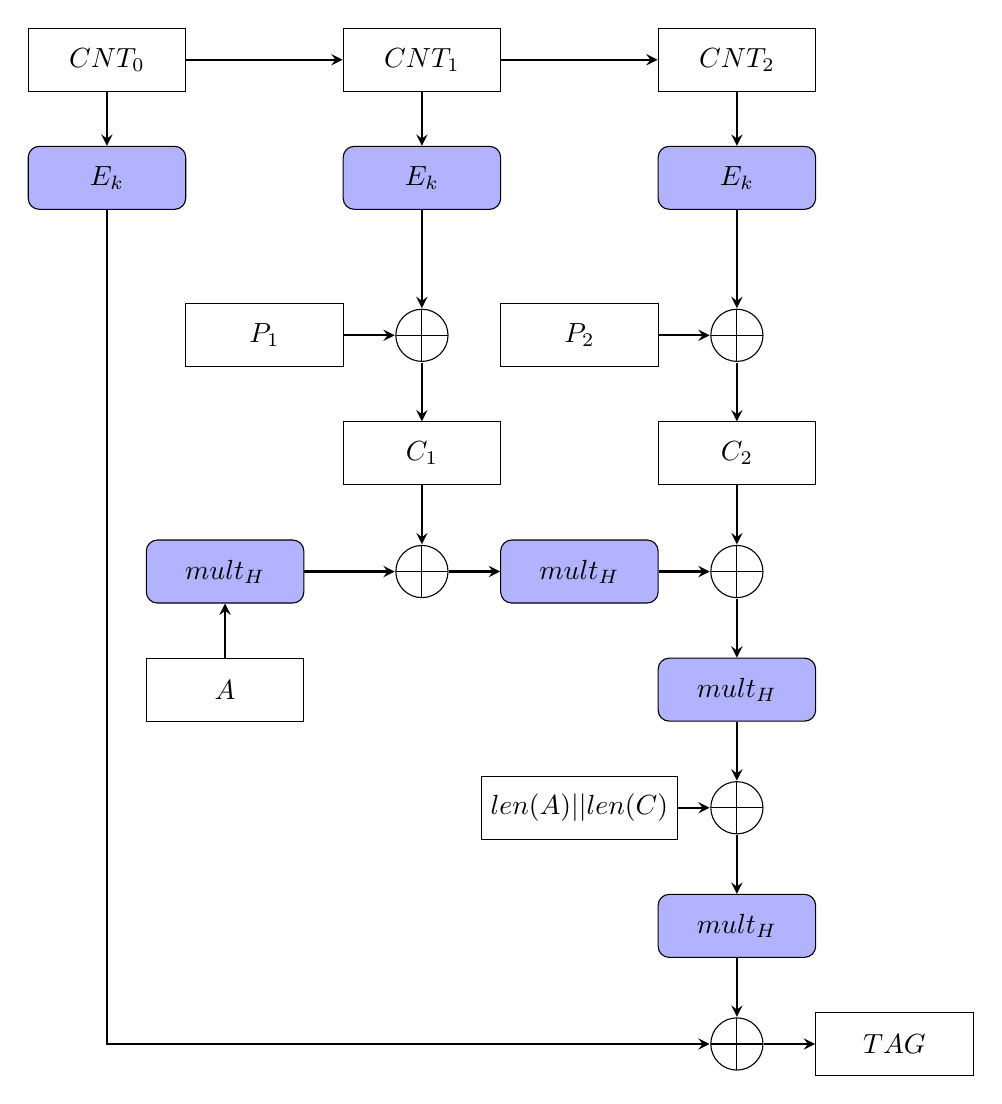
\begin{tikzpicture}
    \node (cnt0) [block]  {$CNT_0$};
    \node (cnt1) [block, right of=cnt0, xshift=3cm]  {$CNT_1$};
    \node (cnt2) [block, right of=cnt1, xshift=3cm]  {$CNT_2$};
    \node (enc0) [function, below of=cnt0, yshift=-0.5cm] {$E_k$};
    \node (enc1) [function, below of=cnt1, yshift=-0.5cm] {$E_k$};
    \node (enc2) [function, below of=cnt2, yshift=-0.5cm] {$E_k$};
    \node (xor11) [XOR, below of=enc1, scale=2, yshift=-0.5cm] {};
    \node (xor12) [XOR, below of=enc2, scale=2, yshift=-0.5cm] {};
    \node (pt1) [block, left of=xor11, xshift=-1cm] {$P_1$};
    \node (pt2) [block, left of=xor12, xshift=-1cm] {$P_2$};
    \node (ct1) [block, below of=xor11, yshift=-0.5cm] {$C_1$};
    \node (ct2) [block, below of=xor12, yshift=-0.5cm] {$C_2$};
    \node (xor21) [XOR, below of=ct1, scale=2, yshift=-0.25cm] {};
    \node (xor22) [XOR, below of=ct2, scale=2, yshift=-0.25cm] {};
    \node (mult1) [function, left of=xor21, xshift=-1.5cm] {$mult_H$};
    \node (mult2) [function, right of=xor21, xshift=1cm] {$mult_H$};
    \node (mult3) [function, below of=xor22, yshift=-0.5cm] {$mult_H$};
    \node (auth) [block, below of=mult1, yshift=-0.5cm] {$A$};
    \node (xor31) [XOR, below of=mult3, scale=2, yshift=-0.25cm] {};
    \node (len) [block, left of=xor31, xshift=-1cm] {$len(A) || len(C)$};
    \node (mult4) [function, below of=xor31, yshift=-0.5cm] {$mult_H$};
    \node (xor41) [XOR, below of=mult4, scale=2, yshift=-0.25cm] {};
    \node (tag) [block, right of=xor41, xshift=1cm] {$TAG$};
    
    \draw [arrow] (cnt0) -- (cnt1);
    \draw [arrow] (cnt1) -- (cnt2);
    \draw [arrow] (cnt0) -- (enc0);
    \draw [arrow] (cnt1) -- (enc1);
    \draw [arrow] (cnt2) -- (enc2);
    \draw [arrow] (enc0) |- (xor41);
    \draw [arrow] (enc1) -- (xor11);
    \draw [arrow] (enc2) -- (xor12);
    \draw [arrow] (pt1) -- (xor11);
    \draw [arrow] (pt2) -- (xor12);
    \draw [arrow] (xor11) -- (ct1);
    \draw [arrow] (xor12) -- (ct2);
    \draw [arrow] (ct1) -- (xor21);
    \draw [arrow] (ct2) -- (xor22);
    \draw [arrow] (mult1) -- (xor21);
    \draw [arrow] (auth) -- (mult1);
    \draw [arrow] (xor21) -- (mult2);
    \draw [arrow] (mult2) -- (xor22);
    \draw [arrow] (xor22) -- (mult3);
    \draw [arrow] (mult3) -- (xor31);
    \draw [arrow] (len) -- (xor31);
    \draw [arrow] (xor31) -- (mult4);
    \draw [arrow] (mult4) -- (xor41);
    \draw [arrow] (xor41) -- (tag);
  \end{tikzpicture}
  \caption{Semantics of AES-GCM} \label{fig:aesgcm}
\end{figure}

The encryption for AES-GCM works according to the following steps:

\begin{enumerate}
  \item The initialisation $IV$ of 96 bits is generated.
  \item The counters $CNT_i$ of 128 bits are generated by $CNT_i = IV \parallel
cnt$, where $cnt = (i + 1) \bmod{2^{32}}$, for $i \in\{0 .. n\}$ and $n$
represents the number of plaintext blocks.
  \item The ciphertexts $C_i$ are generated by encrypting the counter values
$CNT_i$ and XORing it to the plaintext $P_i$, as $C_i = P_i \oplus E_k(CNT_i)$.
\end{enumerate}

To get the authentication tag $TAG$ the so-called $GHASH$ function,
$GHASH(H, A, C) = X_{m+n+1}$, is applied. Where, $H$ is the hash key, computed
by encrypting 128 zero bits with the AES block cypher, $C$ is the ciphertext
and $A$ being non-encrypted but authenticated data. Figure~\ref{fig:aesgcm}
shows how the $GHASH$ is computed for one block of authenticated data and two
blocks of plaintext. This happens according to the following steps:

\begin{enumerate}
  \item The Galois field multiplication is applied to the block of
authenticated data. $R_0 = mult_H(A_1)$.
  \item The result of this is XORed to the first ciphertext. The output
of this XOR is again multiplied in the Galois field. $R_1 = mult_H(R_0 \oplus
C_1)$.
  \item This output is then XORed to the second ciphertext and again
multiplied. $R_2 = mult_H(R_1 \oplus C_2)$
  \item Then the length of the authenticated data and the ciphertext is
added. $R_3 = mult_H(R_2 \oplus (len(A) \parallel len(C)))$
  \item To form the tag $TAG$ the hash key is added in the end. $TAG = H \oplus
mult_H(R_3)$.
\end{enumerate}

The authenticated tag $TAG$ can therefore be found by solving the polynomial
$g(X) = A_{1}X^{m+n+1} + \cdots + A_{m}X^{n+2} + C_{1}X^{n+1} + \cdots +
C_{n}X^2 + LX + S$, as $g(H) = TAG$. Where $L$ is the combined length of $A$
and $C$, and $S$ is the nonce plus the counter. We refer to the NIST
standard about AES-GCM~\cite{gcmnist} for more details.

\subsubsection{AES-GCM Implementation in \texttt{openssl}}

Lorem ipsum dolor sit amet, consetetur sadipscing elitr, sed diam nonumy eirmod
tempor invidunt ut labore et dolore magna aliquyam erat, sed diam voluptua. At
vero eos et accusam et justo duo dolores et ea rebum. Stet clita kasd gubergren,
no sea takimata sanctus est Lorem ipsum dolor sit amet.

\subsection{AES-GCM Nonce Reuse Attack}

In cryptography, the uniqueness of nonces is usually seen as given. Therefore,
Joux~\cite{NISTGCMcomment} calls his attack against GCM "a forbidden attack".
Böck~\etal~\cite{gcmnonceattack} describe how relevant nonce reuse still is in
real-world application and why clear definitions for nonces in protocols
are needed.

To understand the attack by Joux~\cite{NISTGCMcomment}, we look at the
simplified attack, described by Böck~\etal~\cite{gcmnonceattack}. We assume
that the same nonce is used for two messages.

\[
  g_1(X) = C{_{1}X^2 \oplus L_1X \oplus S}
\]

\[
  g_2(X) = C{_{2}X^2 \oplus L_2X \oplus S}
\]

We assume that all values besides $S$ are known to the attacker. We can also
add the known tag $TAG$ to each polynomial to get $g_i'(X)$ as follows:

\[
  g_1'(X) = C{_{1}X^2 \oplus L_1X \oplus S \oplus T_1}
\]

\[
  g_2'(X) = C{_{2}X^2 \oplus L_2X \oplus S \oplus T_2}
\]

The combination of those two can be done, because we know they are equal to
zero, at the point $H$. $g_1'(H) = g_2'(H) = 0$. This combination results in
the following solvable polynomial:

\[
  g_{1+2}'(X) = (C_{1} + C_{2})X^2 + (L_1 + L_2)X + T_1 + T_2
\]

Which is know to fulfil the equation $g_{1+2}'(H) = 0$. Therefore an attacker
can recover a list of candidates for $H$. An increasing number of nonce
reuse lowers the number of possible key candidates.

\todo{Simplify Attack}

\section{Rowhammer}

Technology is steadily changing, with vendors of computer parts being forced to
produce cheaper and hardware every year. For DRAM this resulted in less quality
management and proper checks on possible bitflips which allowed smaller chipsets
into production. These chips provide less space to store loads, which represents
data, and little energy to be used to store the loads. Years after vendors
introduced this increased densities in DRAM to the market researchers like
\todo{references rowhammer} found a critical bug in the chip design. With the
little space and energy stored it was possible to use charges of memory rows to
leak data to nearby rows, which made it possible to even change bits of other
rows with particular crafted memory access patterns like shown by
\todo{references rowhammer}.

This behaviour and bug then caused researchers to dig deeper into the
possibilities, and several attacks were found based on the Rowhammer bug. For
example as~\todo{reference rowhammer exploit} shows, it is possible to use
Rowhammer for privilege escalation.~\todo{reference dramma} also state that this
attack not only affects desktop computers but also memory in mobile devices. In
their work~\todo{reference rowhammer work} show that flipping bits in memory has
further risks as previously thought and that Rowhammer defences need a general
overhaul, stating that the only proper solution is to fix the hardware.
%}}}

%% vim:foldmethod=expr
%% vim:fde=getline(v\:lnum)=~'^%%%%\ .\\+'?'>1'\:'='
%%% Local Variables:
%%% mode: latex
%%% mode: auto-fill
%%% mode: flyspell
%%% eval: (ispell-change-dictionary "en_US")
%%% TeX-master: "main"
%%% End:
